\chapter{Release 2 : Intégration des données "ETL" et gestion multi-domaines}
\minitoc
 \newpage
 \counterwithin{figure}{chapter}
\section{Introduction}
Dans cette deuxième release, la plateforme évolue vers une dimension décisionnelle plus avancée, en intégrant des mécanismes de traitement et d'exploitation des données.
Après avoir mis en place les bases fonctionnelles liées à l'authentification et à la gestion des utilisateurs dans la Release 1, cette phase introduit deux axes majeurs : l'intégration des données via un processus ETL (Extract, Transform, Load), présentée dans la section \ref{sec:Sprint3:ETL}, et la gestion multi-domaines, détaillée dans la section \ref{sec:Sprint4:MultiDomain}.
Ce chapitre présente les différents sprints réalisés, en s'appuyant sur les backlogs et les user stories. Chaque sprint est structuré autour d'une analyse fonctionnelle, suivie d'une conception basée sur des diagrammes de séquence, puis d'une présentation des interfaces réalisées.

\section{Sprint 3 : Intégration des données "ETL"}
\label{sec:Sprint3:ETL}
Dans le cadre de ce projet, le processus d'intégration des données repose sur une approche hybride. En effet, en l'absence de sources de données réelles, nous avons procédé à la génération de jeux de données simulés afin de reproduire un environnement proche de la réalité et de permettre le bon fonctionnement et la validation des différentes fonctionnalités de la plateforme. Cette génération de données a permis de modéliser plusieurs entités, garantissant ainsi la disponibilité d'un volume de données suffisant pour les traitements analytiques.
Par ailleurs, la plateforme ne se limite pas à ces données statiques : l'administrateur dispose également d'un module d'importation lui permettant d'intégrer des données externes à travers plusieurs étapes structurées. Le processus se fait à travers plusieurs étapes afin d'assurer leur cohérence et leur conformité avec le modèle du système. Les données validées sont alors intégrées dans la base de données pour être exploitées par les différents modules analytiques.
Ainsi, cette approche combinant génération de données et import contrôlé permet d'assurer la flexibilité, la robustesse et l'évolutivité du système, tout en garantissant un environnement adapté aux besoins de test et de simulation de la plateforme.

\subsection{Le backlog du sprint 3}
Chaque user story est formulée selon le format « En tant que… je veux… afin de… ». Dans cette partie, nous présentons le backlog du sprint 3, élaboré à partir des besoins fonctionnels identifiés pour le module d'intégration des données. Ce backlog comprend les user stories détaillées permettant de planifier et de prioriser les tâches de ce sprint, comme le montre le tableau \ref{tab:sprint3_backlog}.

\begin{table}[H]
\centering
\caption{Backlog du Sprint 3 : Intégration des données (ETL)}
\label{tab:sprint3_backlog}
\begin{tabular}{|c|p{3.5cm}|p{10cm}|c|}
\hline
\textbf{ID} & \textbf{Fonctionnalité} & \textbf{User Story} & \textbf{Priorité} \\
\hline
\multirow{9}{*}{3} & \multirow{9}{*}{Import de données} 
& En tant qu'administrateur, je veux sélectionner l'entité cible parmi les entités disponibles afin de déterminer dans quelle table les données seront importées. & Must \\
\cline{3-4}
& & En tant qu'administrateur, je veux sélectionner un fichier de données (CSV, excel,xlsx) correspondant à l'entité choisie afin d'importer de nouvelles données dans le système. & Must \\
\cline{3-4}
& & En tant qu'administrateur, je veux que le système détecte automatiquement les correspondances entre les colonnes du fichier et les champs de l'entité cible afin d'accélérer le mapping. & Must \\
\cline{3-4}
& & En tant qu'administrateur, je veux pouvoir ajuster manuellement le mapping des colonnes en cas de correspondance inexacte afin d'assurer la fiabilité de l'import. & Must \\
\cline{3-4}
& & En tant qu'administrateur, je veux visualiser un aperçu des données importées avant validation afin de vérifier leur conformité avec la structure de l'entité sélectionnée. & Must \\
\cline{3-4}
& & En tant qu'administrateur, je veux être notifié en cas d'erreur de format, de type de données incorrect ou de champs obligatoires manquants lors de l'import afin de corriger le fichier source. & Must \\
\cline{3-4}
& & En tant qu'administrateur, je veux lancer le processus d'intégration ETL afin que les données importées soient automatiquement nettoyées, validées et insérées dans la base. & Must \\
\cline{3-4}
& & En tant qu'administrateur, je veux recevoir un rapport détaillé des lignes importées, des erreurs et des doublons détectés afin d'auditer la qualité de l'import. & Should \\
\cline{3-4}
& & En tant qu'administrateur, je veux pouvoir annuler ou corriger une importation en cas d'erreur détectée après coup afin de maintenir l'intégrité des données. & Should \\
\hline
\end{tabular}
\end{table}

\subsection{Analyse}
À partir du backlog du sprint 3, nous détaillons dans la section suivante l'analyse du cas d'utilisation principal « Importer des données ». Cette analyse permet de définir les interactions fonctionnelles entre l'administrateur et le système lors du processus d'intégration des données, prenant en charge les différentes entités disponibles, 

\textbf{Amélioration du cas d'utilisation « Importer des données » :}

La figure \ref{fig:use_case_import} illustre le diagramme de cas d'utilisation présentant les différentes interactions entre l'administrateur et le système lors du processus d'import.

\begin{figure}[H]
    \centering
    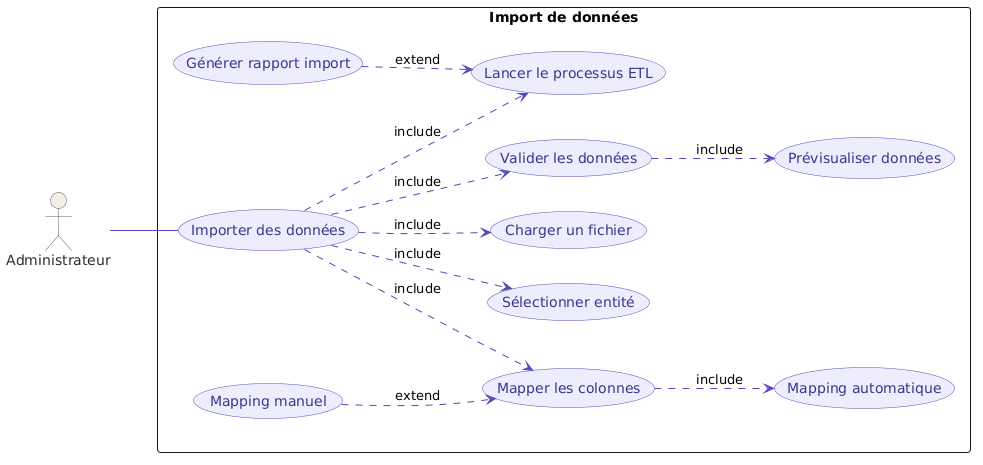
\includegraphics[width=1\textwidth]{project/images/use_case_import.png}
    \caption{Diagramme de cas d'utilisation « Importer des données »}
    \label{fig:use_case_import}
\end{figure}

Le tableau \ref{tab:import_donnees} présente la description textuelle du cas d'utilisation « Importer des données ».

\begin{longtable}{|l|p{12cm}|}
\caption{Cas d'utilisation – Import de données}
\label{tab:import_donnees} \\
\hline
\textbf{Élément} & \textbf{Description} \\
\hline
\endfirsthead
\hline
\textbf{Élément} & \textbf{Description} \\
\hline
\endhead

Cas d'utilisation & 
\begin{itemize}
    \item Importer des données
\end{itemize} \\
\hline
Acteur & 
\begin{itemize}
    \item Administrateur
\end{itemize} \\
\hline
Préconditions & 
\begin{itemize}
    \item L'administrateur est authentifié et possède les droits d'import
    \item Le système est fonctionnel et la base de données accessible
    \item Au moins une entité d'import est configurée dans le système
    \item Un fichier de données est disponible
\end{itemize} \\
\hline
Scénario de base & 
\textbf{Scénario 1 : Sélection de l'entité cible} \\
&-L'administrateur accède au module d'import. \\
&-Le système affiche la liste des entités disponibles. \\
&-L'administrateur sélectionne l'entité cible. \\
&-Le système récupère les informations de l'entité sélectionnée. \\
&-Le système affiche l'interface de sélection de fichier adaptée à l'entité. \\
\\
& \textbf{Scénario 2 : Sélection et chargement du fichier} \\
&-L'administrateur sélectionne un fichier (CSV ou Excel). \\
&-Le système vérifie que l'extension du fichier correspond au format attendu. \\
&-Le système vérifie que la taille du fichier ne dépasse pas la limite autorisée. \\
&-Le système charge et parse le fichier. \\
&-Le système extrait les en-têtes de colonnes du fichier. \\
\\
& \textbf{Scénario 3 : Mapping automatique des colonnes} \\
&-Le système compare les en-têtes du fichier avec les champs définis dans le modèle de données. \\
&-En cas de correspondance exacte, le système pré-remplit le mapping automatiquement. \\
&-Le système affiche le mapping proposé à l'administrateur. \\
\\
& \textbf{Scénario 4 : Mapping manuel (si nécessaire)} \\
&-L'administrateur visualise les colonnes non mappées ou mal mappées. \\
&-L'administrateur sélectionne manuellement dans une liste déroulante le champ de la base correspondant à chaque colonne du fichier. \\
&-L'administrateur valide le mapping final. \\
&-Le système vérifie que tous les champs obligatoires de l'entité sont couverts. \\
\\
& \textbf{Scénario 5 : Aperçu des données (Preview)} \\
&-Le système affiche un aperçu des premières lignes du fichier avec le mapping appliqué. \\
&-L'administrateur vérifie visuellement la conformité des données. \\
\\
& \textbf{Scénario 6 : Validation des données} \\
&-Le système vérifie la conformité des types de données. \\
&-Le système détecte les valeurs manquantes sur les champs obligatoires. \\
&-Le système identifie les doublons potentiels (basés sur les champs uniques comme l'email). \\
&-Le système affiche les erreurs détectées avec indication des lignes concernées. \\
&-L'administrateur corrige les erreurs ou choisit d'ignorer les lignes invalides. \\
\\
& \textbf{Scénario 7 : Traitement ETL} \\
&-L'administrateur lance le processus d'intégration. \\
&-Le système effectue le nettoyage des données. \\
&-Le système transforme les données selon les règles métier de l'entité. \\
&-Le système détecte et gère les doublons (fusion ou rejet). \\
&-Le système insère les données validées dans la table correspondante de la base de données. \\
&-Le système met à jour les logs d'audit avec l'identifiant de l'administrateur et la date. \\
\\
& \textbf{Scénario 8 : Rapport d'import} \\
&-Le système génère un rapport indiquant le nombre de lignes importées et en erreur. \\
&-Le système affiche un message de confirmation à l'administrateur. \\
\\
& \textbf{Scénario 9 : Gestion des erreurs (Rollback)} \\
&-En cas d'erreur lors de l'insertion en base de données, le système effectue un rollback de la transaction en cours. \\
&-Les données en cours d'import sont annulées. \\
& Le système notifie l'administrateur de l'échec de l'opération. \\
\hline
Scénarios alternatifs & 
\textbf{1.1 Entité non configurée :} Si l'entité sélectionnée n'a pas de structure définie, le système affiche un message d'erreur et invite à contacter le support technique. \\
& \textbf{2.1 Format de fichier invalide :} Si le fichier n'est pas compatible ou dépasse la taille maximale autorisée, un message d'erreur s'affiche et l'administrateur doit sélectionner un autre fichier. \\
& \textbf{2.2 Fichier vide :} Si le fichier ne contient aucune donnée ou aucun en-tête, le système affiche un avertissement et empêche la poursuite du processus. \\
& \textbf{3.1 Aucune correspondance automatique :} Si aucun en-tête ne correspond aux champs de l'entité, le système passe directement au mapping manuel avec une alerte informative. \\
& \textbf{4.1 Champs obligatoires non mappés :} Si des champs obligatoires de l'entité ne sont pas couverts par le mapping, le système bloque la validation et demande à l'administrateur de compléter. \\
& \textbf{6.1 Erreurs bloquantes :} Si des erreurs critiques sont détectées, l'import est bloqué jusqu'à correction du fichier. \\
& \textbf{9.1 Échec technique durant l'import :} Si une erreur survient lors de l'insertion en base de données, le système effectue un rollback automatique de la transaction en cours. Toutes les données de l'import sont annulées et le statut passe à « Échoué ». \\
\hline
Post-conditions & 
\begin{itemize}
    \item Les données validées sont intégrées dans la table de l'entité sélectionnée.
    \item Le statut du job d'import est mis à jour dans la table \texttt{import\_job}
    \item Les logs d'audit sont mis à jour avec les actions de l'administrateur.
\end{itemize} \\
\hline
\end{longtable}

\subsection{Conception}
Dans cette partie, nous présentons la conception du cas d'utilisation « Importer des données » à travers un diagramme de séquence. Ce diagramme illustre les interactions entre l'administrateur et les différents composants du système lors du processus d'importation des données, en mettant en évidence les étapes clés telles que la sélection de l'entité, le mapping des colonnes, la validation des données et le traitement ETL.
La figure \ref{fig:seqdiagram_import} illustre le diagramme de séquence présentant les différentes interactions entre l'administrateur et le système lors du processus d'import.
\begin{figure}[H]
    \centering
    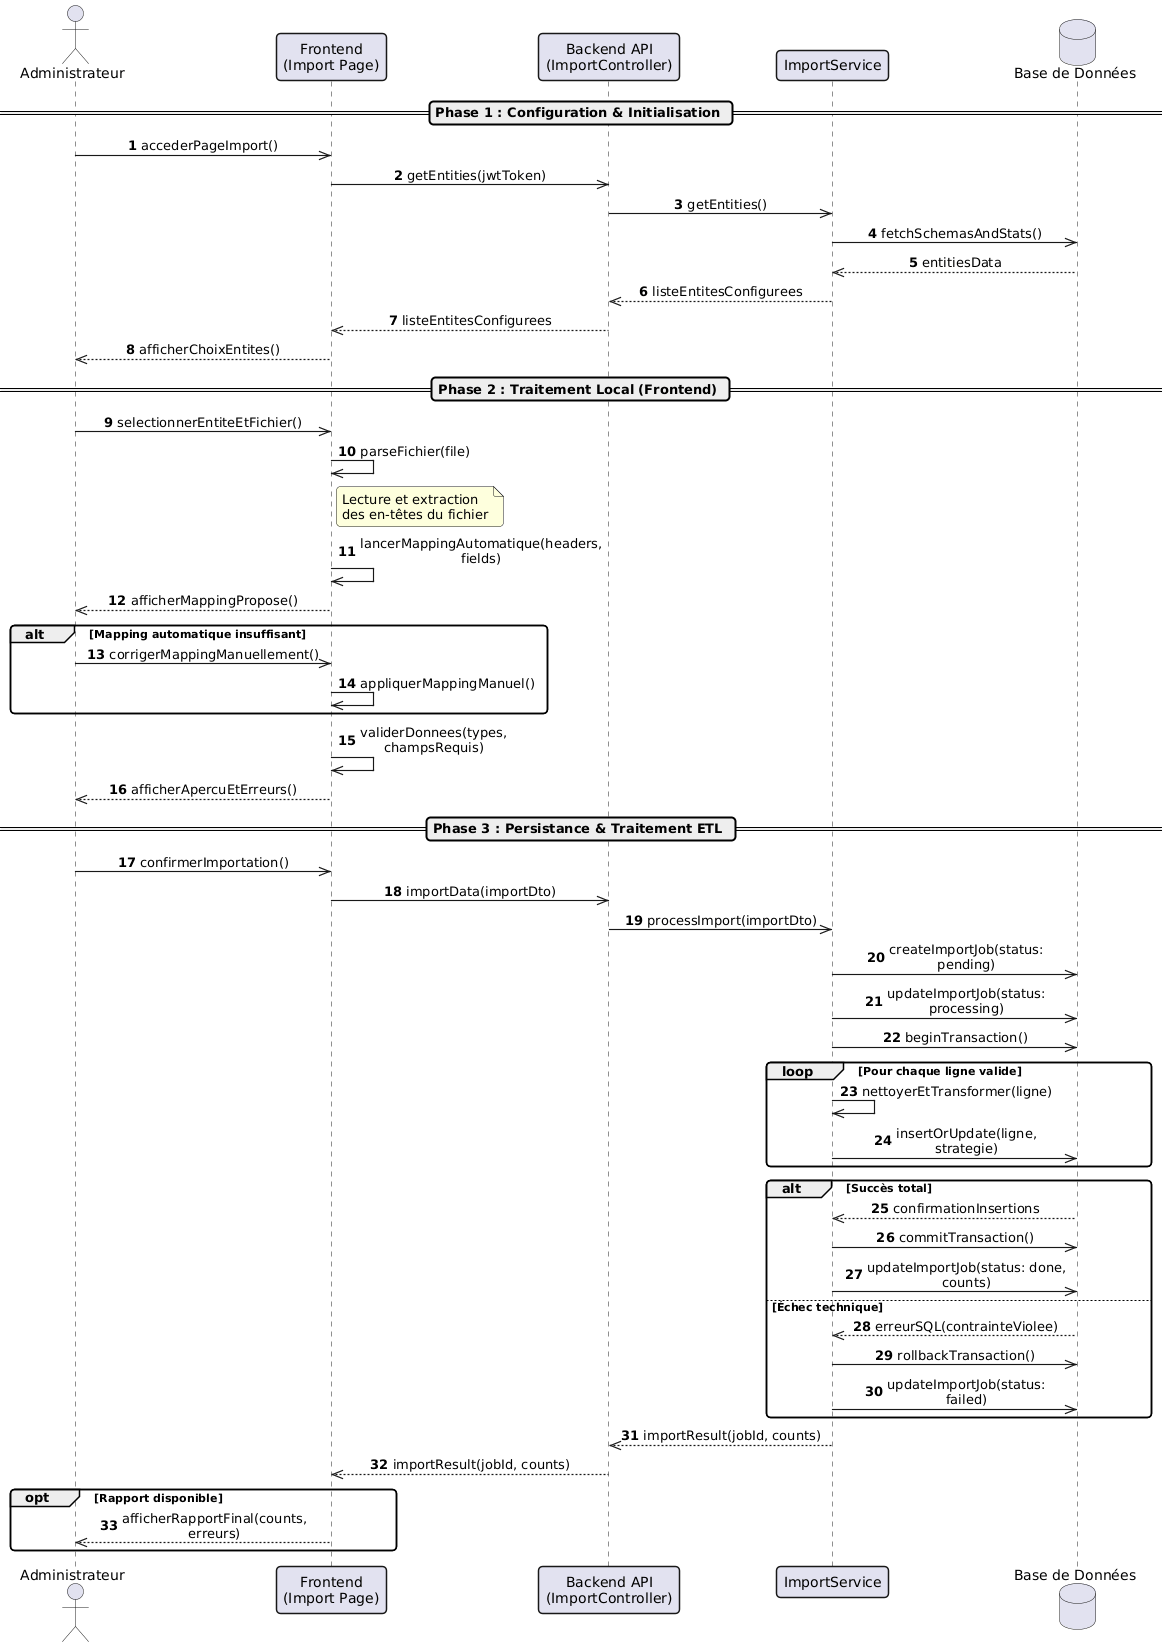
\includegraphics[width=0.9\textwidth]{project/images/seqdiagram_import.png}
    \caption{Diagramme de séquence « Importer des données »}
    \label{fig:seqdiagram_import}
\end{figure}

\subsection{Réalisation}
Dans cette section, nous présentons les interfaces réalisées pour le module d'importation des données, en mettant l'accent sur les différentes étapes du processus d'intégration. Les captures d'écran suivantes illustrent les écrans de sélection de l'entité cible, de mapping des colonnes, d'aperçu des données et de rapport d'import.



\section{Sprint 4 : Gestion multi-domaines}
\label{sec:Sprint4:MultiDomain}
Comme perspectives, nous proposons...